\subsection{Proceso Interno 04: Crear Nueva Simulación}

\subsubsection{Objetivo del Proceso}
Instanciar un entorno de simulación vacío usando REBOUND, preparado para:
\begin{itemize}
    \item Configuración posterior de parámetros
    \item Simulación de dinámica gravitacional de 2 cuerpos
    \item Cálculo del Exponente de Lyapunov (LE)
\end{itemize}

\subsubsection{Entradas Principales}
\begin{itemize}
    \item \textbf{Trigger}: Señal de solicitud de creación
    \item \textit{Nota}: No se requieren datos específicos de entrada
\end{itemize}

\subsubsection{Sub-pasos Secuenciales}
Este apartado es proporcionado para profundizar y describir de forma textual cada paso contenido dentro del diagrama del proceso descrito en la figura~\ref{fig:process_diagram04}
\subsubsection*{1. Invocar API de REBOUND}
\begin{verbatim}
sim = rebound.Simulation()
\end{verbatim}

\subsubsection*{2. Inicialización Interna}
REBOUND ejecuta:
\begin{itemize}
    \item Asignación de memoria para estructura \texttt{Simulation}
    \item Creación de contenedor vacío para partículas
    \item Configuración de valores por defecto:
    \begin{itemize}
        \item $t_0 = 0$
        \item $G = 6.674\times10^{-11}\ \text{N·m}^2/\text{kg}^2$
        \item Integrador: \texttt{WHFast}
    \end{itemize}
\end{itemize}

\subsubsection*{3. Generar Referencia}
\begin{itemize}
    \item Retorna handler/puntero: \texttt{Simulation*}
    \item Ejemplo: \texttt{0x7ffe3c3d8b50} %chktex 29
\end{itemize}

\subsubsection*{4. Transferir Control}
\begin{itemize}
    \item Pasa referencia al proceso ``Definir Condiciones''
\end{itemize}

\subsubsection{Lógica Interna y Decisiones}
\begin{itemize}
    \item \textbf{Flujo lineal}: Sin bifurcaciones condicionales
    \item \textbf{Manejo de errores}:
    \begin{itemize}
        \item Excepciones de API manejadas en nivel superior
    \end{itemize}
    \item \textbf{Defaults}:
    \begin{itemize}
        \item Valores modificables en configuración posterior
    \end{itemize}
\end{itemize}

\subsubsection{Manejo de Datos Específico}
\begin{itemize}
    \item \textbf{Entrada}: Solo trigger de activación
    \item \textbf{Intermedios}:
    \begin{itemize}
        \item Estructura \texttt{Simulation} en memoria
        \item Estado inicial: $t=0$, $\text{partículas}=\emptyset$
    \end{itemize}
    \item \textbf{Salida}: Referencia a \texttt{Simulation}
\end{itemize}

\subsubsection{Salidas Principales}
\begin{itemize}
    \item \texttt{Simulation*}: Puntero a instancia REBOUND vacía
    \begin{itemize}
        \item Lista para configuración de parámetros
        \item Integrable en flujo de optimización
    \end{itemize}
\end{itemize}

\subsubsection{Interacciones Internas}
\begin{itemize}
    \item \textbf{Con API REBOUND}:
    \begin{itemize}
        \item Constructor \texttt{rebound.Simulation~()}
        \item Gestión interna de memoria
    \end{itemize}
    \item \textbf{Con subsistema de memoria}:
    \begin{itemize}
        \item Asignación dinámica (~KB a MB según complejidad)
    \end{itemize}
    \item \textbf{Con flujo de control}:
    \begin{itemize}
        \item Paso de referencia a siguiente módulo
    \end{itemize}
\end{itemize}
\newpage
\subsubsection{Diagrama del Proceso}
\begin{figure}[H]
    \centering
    \adjustbox{max width=\textwidth, max height=0.9\textheight}{%
        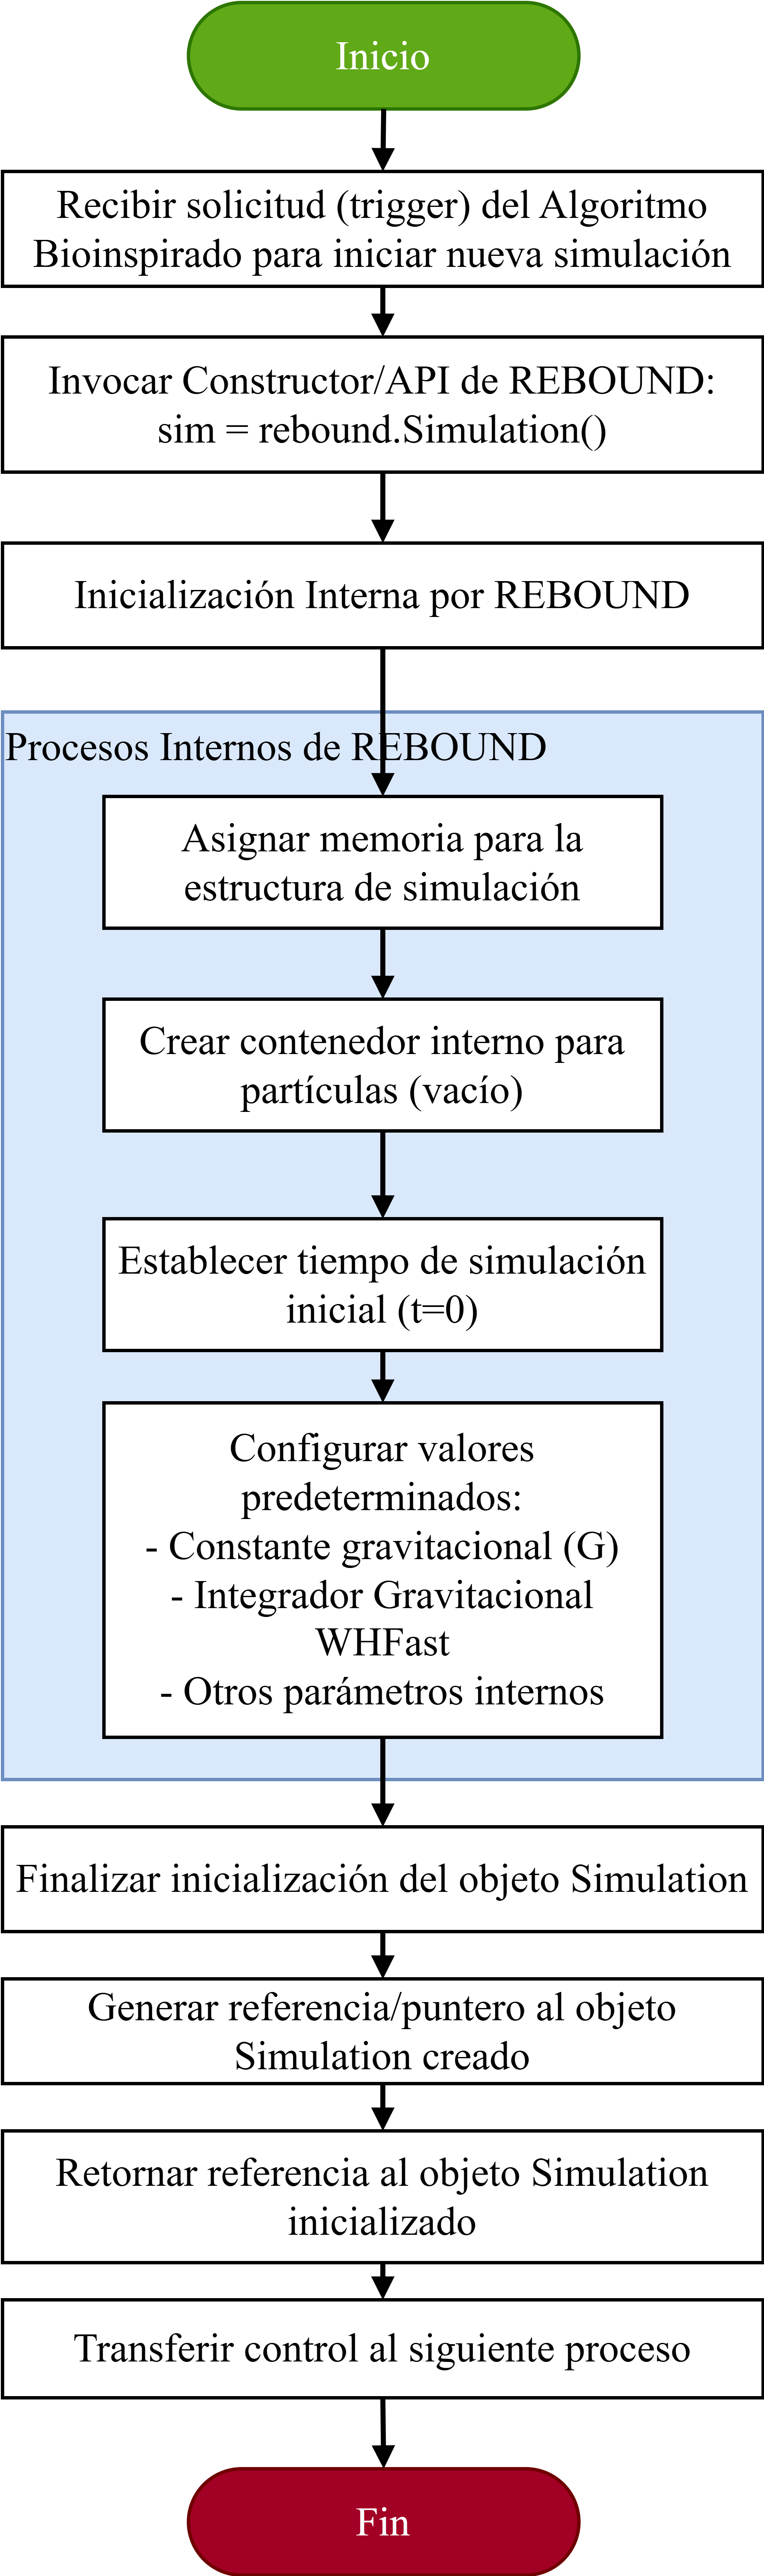
\includegraphics[width=\textwidth]{img/Analisis/DiagramaProcesos/DiagramaProceso04_CrearSimulacion.png}
    }
        \caption{Diagrama de Proceso Interno 04: Crear Simulación}%
    \label{fig:process_diagram04}
\end{figure}
\newpage